\documentclass[journal,twoside,web]{ieeecolor}
\usepackage{generic}
\usepackage{cite}
\usepackage{amsmath,amssymb,amsfonts}
\usepackage{algorithmic}
\usepackage{graphicx}
\usepackage{algorithm,algorithmic}
\usepackage{hyperref}
\usepackage{booktabs}
\hypersetup{hidelinks=true}
\usepackage{textcomp}
\def\BibTeX{{\rm B\kern-.05em{\sc i\kern-.025em b}\kern-.08em
    T\kern-.1667em\lower.7ex\hbox{E}\kern-.125emX}}
\markboth{\hskip25pc IEEE TRANSACTIONS AND JOURNALS TEMPLATE}
{Author \MakeLowercase{\textit{et al.}}: Title}
\begin{document}
\title{Preparation of Papers for IEEE Transactions and Journals (June 2023)}
\author{Armin Berger, Max Möbus, and Third C. Author Jr., \IEEEmembership{Member, IEEE}
\thanks{This paragraph of the first footnote will contain the date on 
which you submitted your paper for review. It will also contain support 
information, including sponsor and financial support acknowledgment. For 
example, ``This work was supported in part by the U.S. Department of 
Commerce under Grant 123456.'' }
\thanks{The next few paragraphs should contain 
the authors' current affiliations, including current address and e-mail. For 
example, First A. Author is with the National Institute of Standards and 
Technology, Boulder, CO 80305 USA (e-mail: author@boulder.nist.gov). }
\thanks{Second B. Author Jr. was with Rice University, Houston, TX 77005 USA. He is 
now with the Department of Physics, Colorado State University, Fort Collins, 
CO 80523 USA (e-mail: author@lamar.colostate.edu).}
\thanks{Third C. Author is with 
the Electrical Engineering Department, University of Colorado, Boulder, CO 
80309 USA, on leave from the National Research Institute for Metals, 
Tsukuba, Japan (e-mail: author@nrim.go.jp).}}

\maketitle

\begin{abstract}
These instructions give you guidelines for preparing papers for 
IEEE Transactions and Journals. Use this document as a template if you are 
using \LaTeX. Otherwise, use this document as an 
instruction set. The electronic file of your paper will be formatted further 
at IEEE. Paper titles should be written in uppercase and lowercase letters, 
not all uppercase. Avoid writing long formulas with subscripts in the title; 
short formulas that identify the elements are fine (e.g., "Nd--Fe--B"). Do 
not write ``(Invited)'' in the title. Full names of authors are preferred in 
the author field, but are not required. Put a space between authors' 
initials. The abstract must be a concise yet comprehensive reflection of 
what is in your article. In particular, the abstract must be self-contained, 
without abbreviations, footnotes, or references. It should be a microcosm of 
the full article. The abstract must be between 150--250 words. Be sure that 
you adhere to these limits; otherwise, you will need to edit your abstract 
accordingly. The abstract must be written as one paragraph, and should not 
contain displayed mathematical equations or tabular material. The abstract 
should include three or four different keywords or phrases, as this will 
help readers to find it. It is important to avoid over-repetition of such 
phrases as this can result in a page being rejected by search engines. 
Ensure that your abstract reads well and is grammatically correct.
\end{abstract}

\begin{IEEEkeywords}
Enter key words or phrases in alphabetical order, separated by commas. Using the IEEE Thesaurus can help you find the best standardized keywords to fit your article. Use the thesaurus access request form for free access to the IEEE Thesaurus: \underline{https://www.ieee.org/publications/services/thesaurus-acce}\\
\underline{ss-page.com.}
\end{IEEEkeywords}

\section{Introduction}
\label{sec:introduction}


\section{Related Work}
- Introduce harnet10

\section{Method}
\subsection{Overview}
\subsection{Problem Formulation}
NETWORK-NAME is designed to solve the problem of predicting the sleep stage for an interval of accelerometer data. The input is a time-contiguous sequence of $P+1$ windows, where the last window is the causal variable. Thus, the input has dimensionality $P+1 \times C \times S$, where $C$ is the number of channels and $S$ is the number of samples per window. The label is taking values in $\{0,1,2\}$, each matching the sleep stages \textit{Wake}, \textit{NREM}, and \textit{REM} respectively. Here \textit{N1}, \textit{N2}, and \textit{N3}, according to the AASM sleep standard \cite{aasm}, are grouped into a single class \textit{NREM}.

The number of windows $P$ is chosen to contain $L$ minutes of accelerometer recordings and is calculated as $P = \lceil \frac{L \times 60}{W} \rceil$, where $W$ is the window size in seconds. The output of the model is a vector of probabilities for each class, which can be interpreted as the likelihood of each sleep stage for the last window. For all experiments in this paper, $L$ is chosen to be 90 minutes.


% Include info about the training process (lr, optimizer, etc.)
\subsection{Self-supervised Pre-training}
\subsubsection{Backbone Network}
We reused the ResNet-V2 with 18 layers and 1D convolutions from \cite{yuan2022selfsupervised} for the main feature extractor, in order to ensure comparability with the pre-trained \textit{harnet10} model. This network expects inputs with three channels and 300 samples. Its output is a feature vector of size 1024.
\subsubsection{Adaptation of SimCLR Framework}
\begin{figure}
  \centering
  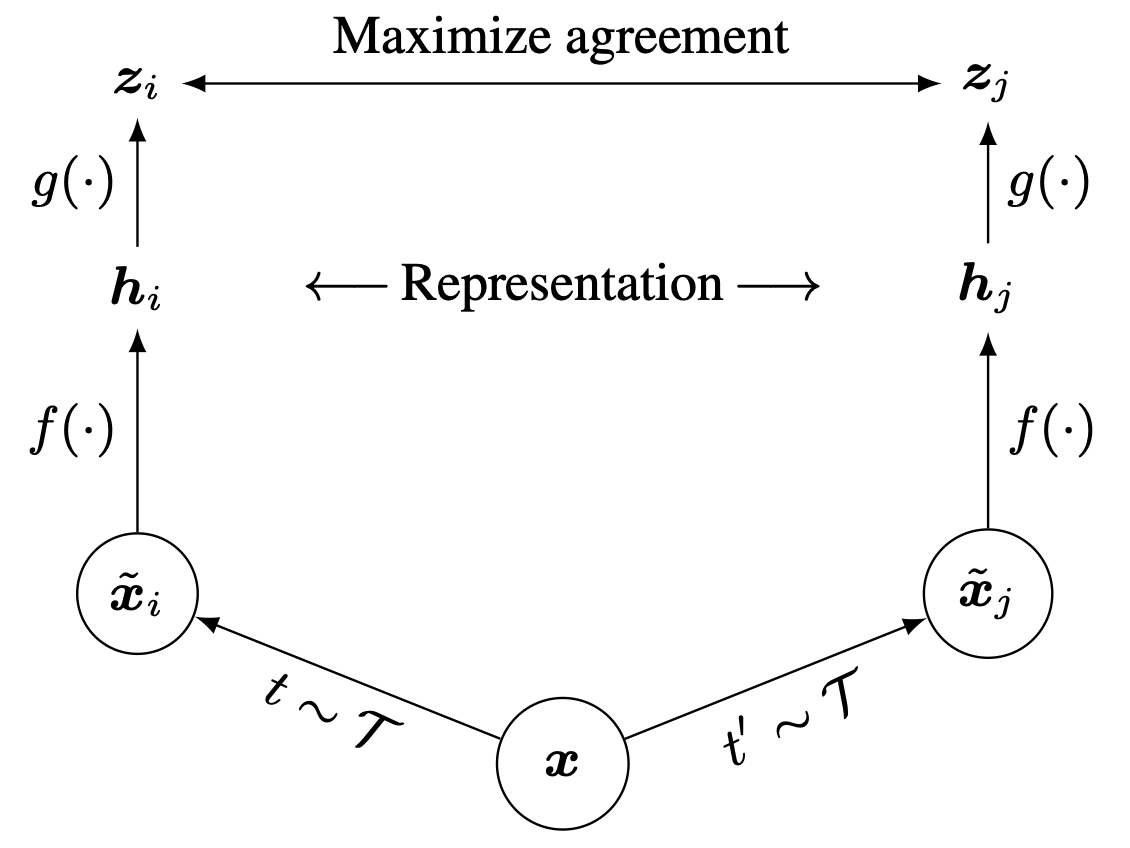
\includegraphics[width=\linewidth]{figures/simclr_overview.png}
  \caption{For each batch two separate data augmentation operators are sampled from the same family of augmentations ($t \sim T$ and $t' \sim T$) and applied to each member of the batch to obtain two correlated views. A feature extractor backbone f(·) and a projection head g(·) are trained to maximize agreement using the NTXentLoss. After training is completed, we throw away the projection head g(·) and use encoder f(·) and its output $h$ for downstream tasks. (Figure and caption adapted from \protect\cite{chen2020simple})}
  \label{fig:simclr_overview}
\end{figure}

For self-supervised learning, we have adapted the SimCLR framework ~\cite{chen2020simple} to use a 1D convolutional backbone. Please refer to Figure \ref{fig:simclr_overview} for a short overview of it. A two-layer feed-forward network with ReLU activation, output size 128, and hidden dimension equal to input size is chosen as the projection head.

\subsubsection{Sleep-staging-specific data augmentations}
We have 17 augmentations that can be chosen for inclusion into the family of augmentations used for training and have used the code from ~\cite{qian2022makes} to implement them. Descriptions of the augmentations can be found in Table \ref{tab:ss_augmentations}.
\begin{table}[h]
  \setlength{\tabcolsep}{1mm}
  \caption{Self-supervised data-augmentation operations used in the SimCLR pipeline.}
  \label{tab:ss_augmentations}
  \centering
  \footnotesize
  \begin{tabular}{|p{18mm}|p{68mm}|}
    \hline
    \textbf{Name} & \textbf{Description} \\ \hline

    na & Returns the window unchanged. \\ \hline

    shuffle & Randomly permutes the channels of the sample. \\ \hline

    jit\_scal & Applies noise and scaling to the sample. \\ \hline

    perm\_jit & Applies permutation and noise to the sample. \\ \hline

    resample & Up-samples the signal on the time axis to $3\times$ its original time steps by linear interpolation and randomly down-samples back to the initial dimensions. \\ \hline

    noise & Adds a randomly generated noise signal with mean $0$ and standard deviation $0.8$. \\ \hline

    scale & Amplifies each channel by a randomly generated distortion with mean $2$ and standard deviation $1.1$. \\ \hline

    negate & Multiplies the value of the signal by $-1$. \\ \hline

    t\_flip & Reverses the signal in the time dimension. \\ \hline

    rotation & Rotates the 3-axial (x, y, z) readings by a random degree uniformly distributed between $-\pi$ and $\pi$ around a random axis in 3D space. \\ \hline

    hfc & Splits the low- and high-frequency components and retains the high-frequency components. \\ \hline

    lfc & Splits the low- and high-frequency components and retains the low-frequency components. \\ \hline

    p\_shift & Shifts the phase values of the frequency response by a random number uniformly distributed between $-\pi$ and $\pi$. \\ \hline

    ap\_p & Perturbs the amplitude and phase values of a randomly selected half-length segment of the frequency response: amplitude is corrupted with Gaussian noise (mean $0$, standard deviation $0.8$) and phase is offset by values uniformly sampled in $[-\pi,\pi]$. \\ \hline

    ap\_f & Applies the same amplitude and phase perturbations as \texttt{ap\_p} to the whole frequency response sequence. \\ \hline

    perm\_harnet & Splits the time axis into exactly four segments with cut points at least $10$ samples apart and permutes the segments. \\ \hline

    t\_warp\_harnet & Warps time per channel using cubic splines and resamples each axis independently. \\ \hline

  \end{tabular}
\end{table}
\subsubsection{Training}
We optimized the model with Adam at a learning rate of $1\times10^{-3}$ using large mini-batches of 2048. Training proceeded for up to 100 epochs, with early stopping triggered by validation loss (patience of 10 epochs); the checkpoint with the lowest validation loss was retained.
\subsection{Sleep-staging Classifier}
% Muss nicht mega detailliert sein, 2-3 sätze reichen
We use the outputs of the pre-trained, frozen backbone network to extract features from the input windows and then stack two bidirectional LSTM layers (1024 units each) to capture temporal dependencies, followed by two fully connected layers (512 units each) that map to the output space. The model is trained to discriminate between all available sleep stages (Wake, N1, N2, N3, REM). For the three-class setting during evaluation, N1–N3 are collapsed into a single NREM class.

We trained the model with Adam (learning rate $1\times10^{-3}$, weight decay $1\times10^{-4}$) using mini-batches of 128 and a class-weighted cross-entropy objective, where weights were the inverse of class frequencies to counter imbalance. To stabilize the LSTMs we applied gradient clipping with a norm of 1. Training proceeded for at most 30 epochs with a five-epoch burn-in before enabling early stopping; early stopping monitored validation cross-entropy with a patience of 10, and the checkpoint with the lowest validation cross-entropy was selected.

Evaluation followed five-fold subject-wise cross-validation. In each fold, subjects were partitioned 80/20 into training and test sets, and the training portion was further split 80/20 to form the final training and validation sets.
\section{Experiments}
\subsection{Datasets and Preprocessing}
\subsubsection{Apple Watch Dataset}
% # participants, dominant wrist, ppg available

The Apple Watch dataset~\cite{walch2019sleep} encompasses information from 31 healthy adults. These participants underwent a Polysomnography (PSG) in line with the American Academy of Sleep Medicine's (AASM) technical specifications, except for the usage of the oronasal thermistor and nasal pressure transducer. Simultaneously, each participant wore an Apple Watch on one wrist. Data from all participants was recorded at a 50 Hz sampling rate with the exception those with IDs 5383425 and 8258170, which we exclude. Thus, the dataset includes data from 29 participants.
\subsubsection{Geneactiv Dataset}
The GENEActive Validation dataset~\cite{van2018estimating} is comprised of data from 22 healthy adults with good sleep habits. They participated in a one-night PSG assessment at the University of Pennsylvania Center for Sleep. All 22 participants from this polysomnography study provided complete accelerometer data from their non-dominant wrist using an Axivity brand accelerometer with a sampling rate of 100 Hz. We exclude participant with ID 1001 for data corruption issues. This yields a total of 21 participants for the GENEActive Validation dataset.
\subsubsection{Newcastle Dataset}
The Newcastle dataset~\cite{vanhees_newcastle_2018} included 28 adult patients who underwent a one-night polysomnography evaluation in a laboratory setting during their regular clinical appointment. Throughout the polysomnography session, participants were equipped with two GENEActive devices, one on each wrist. These wristbands recorded data at a sampling rate of 85.7 Hz. We only used the measurements from the left wrist, because no data on handedness of each participant is included and excluded the data of participant ID 29 because of corruption issues. This yields a total of 27 participants for the Newcastle dataset.
\subsubsection{Chartié Dataset}
The Chartié dataset consists of data from 30 healthy adults who underwent a one-night PSG evaluation. Each participant wore a wrist-worn accelerometer during the PSG session, which recorded data at a sampling rate of 128 Hz. We exclude participants with incomplete motion or PSG data, high clock drift, and invalid labels, resulting in a total of 174 participants for the Chartié dataset.
\subsubsection{Capture24 Dataset}
The Capture-24 dataset~\cite{chan2021capture} features data from Axivity AX3 wrist-worn activity trackers. This data was gathered from 151 participants between 2014 and 2016 in the Oxfordshire region. Recorded at a 100 Hz sampling rate, participants wore the device for approximately 24 hours in their daily routines. This resulted in a cumulative data span of nearly 4,000 hours.
\subsubsection{Data Preprocessing}

We preprocess all raw tri-axial accelerometer streams with the \texttt{actipy} Python package. First, we apply a low-pass filter with a cutoff of 15~Hz to attenuate high-frequency noise, followed by gravity calibration to correct sensor bias and align the static component with standard gravity. The signals are then resampled to 30~Hz to standardize sampling rates across datasets.

After preprocessing, each recording is segmented into non-overlapping windows of length 10~s (i.e., 300 samples per channel at 30~Hz). We discard windows that (i) do not have an accompanying PSG-derived sleep-stage label or (ii) contain any missing values (NaNs). To reduce the impact of motion artifacts and extreme values, we clip per-axis samples whose absolute acceleration exceeds $2\,g$ ($g$ denotes standard gravity). Finally, we normalize each window independently by dividing each channel by its per-window standard deviation, to improve scale invariance across subjects and devices.

\subsection{Baseline Methods}

\subsection{Choosing Augmentations}
To select a subset of the 17 augmentations for our final feature extractor, we performed a systematic evaluation of each augmentation's impact on downstream task performance. This evaluation involved training our model with all two-element combinations of augmentations and assessing their performance in terms of Cohen's kappa. We then selected a four-element combination by hand based on the clustered heatmap.
Through this process we selected \texttt{lfc}, \texttt{rotation}, \texttt{scale}, and \texttt{noise}.


\section{Results}
\begin{figure}[!t]               
  \centering

  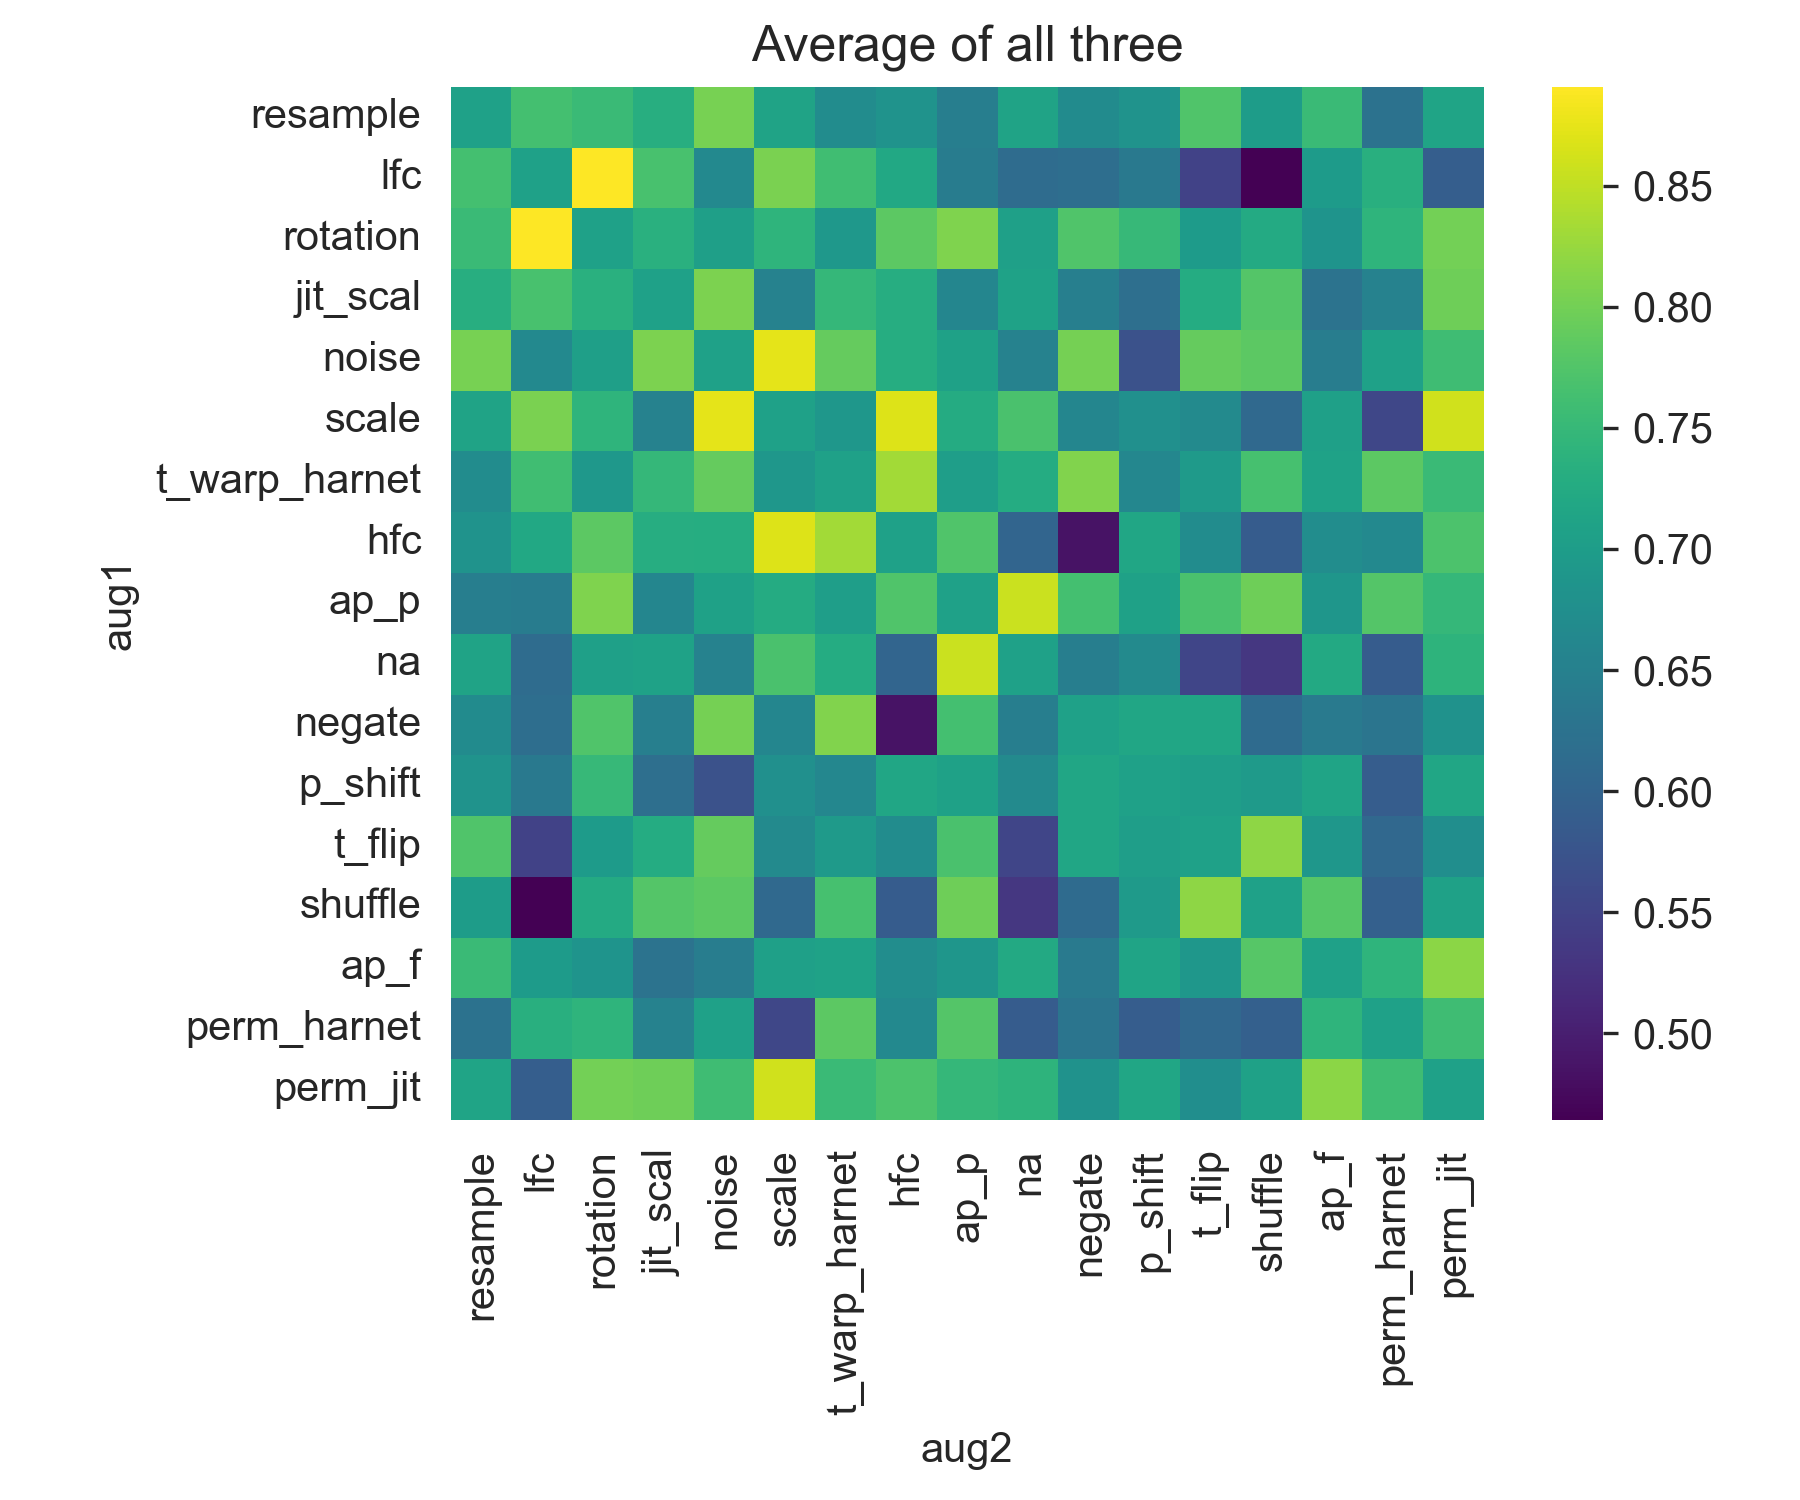
\includegraphics[width=\linewidth]{figures/average_of_all_three.png}  
  \caption{Caption text goes here.}
  \label{fig:example1}    
\end{figure}
\begin{figure}[!t]               
  \centering
  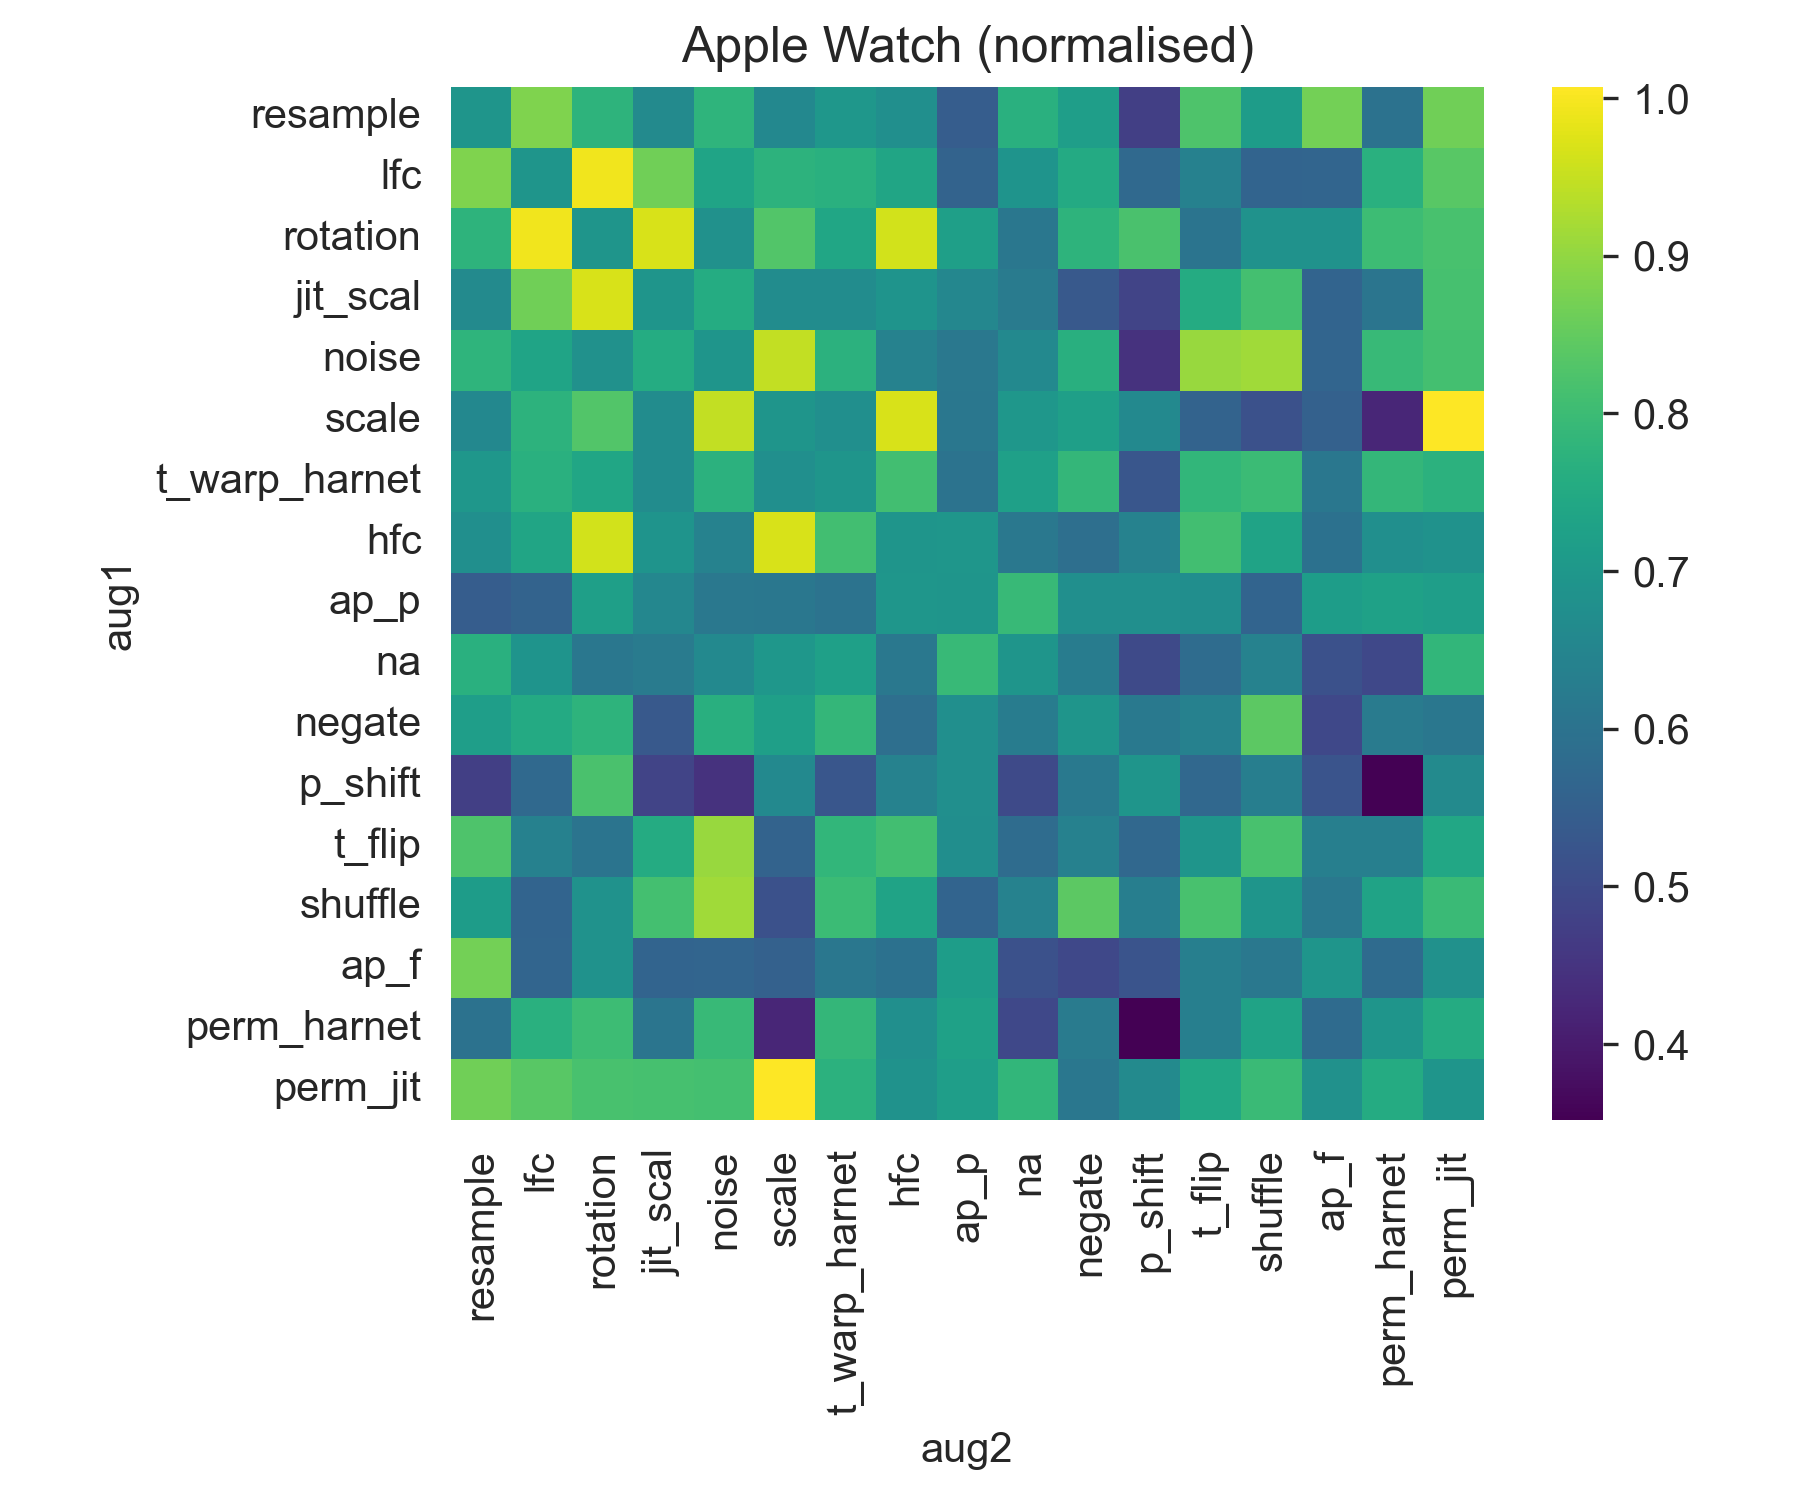
\includegraphics[width=\linewidth]{figures/apple_watch_normalised.png}
  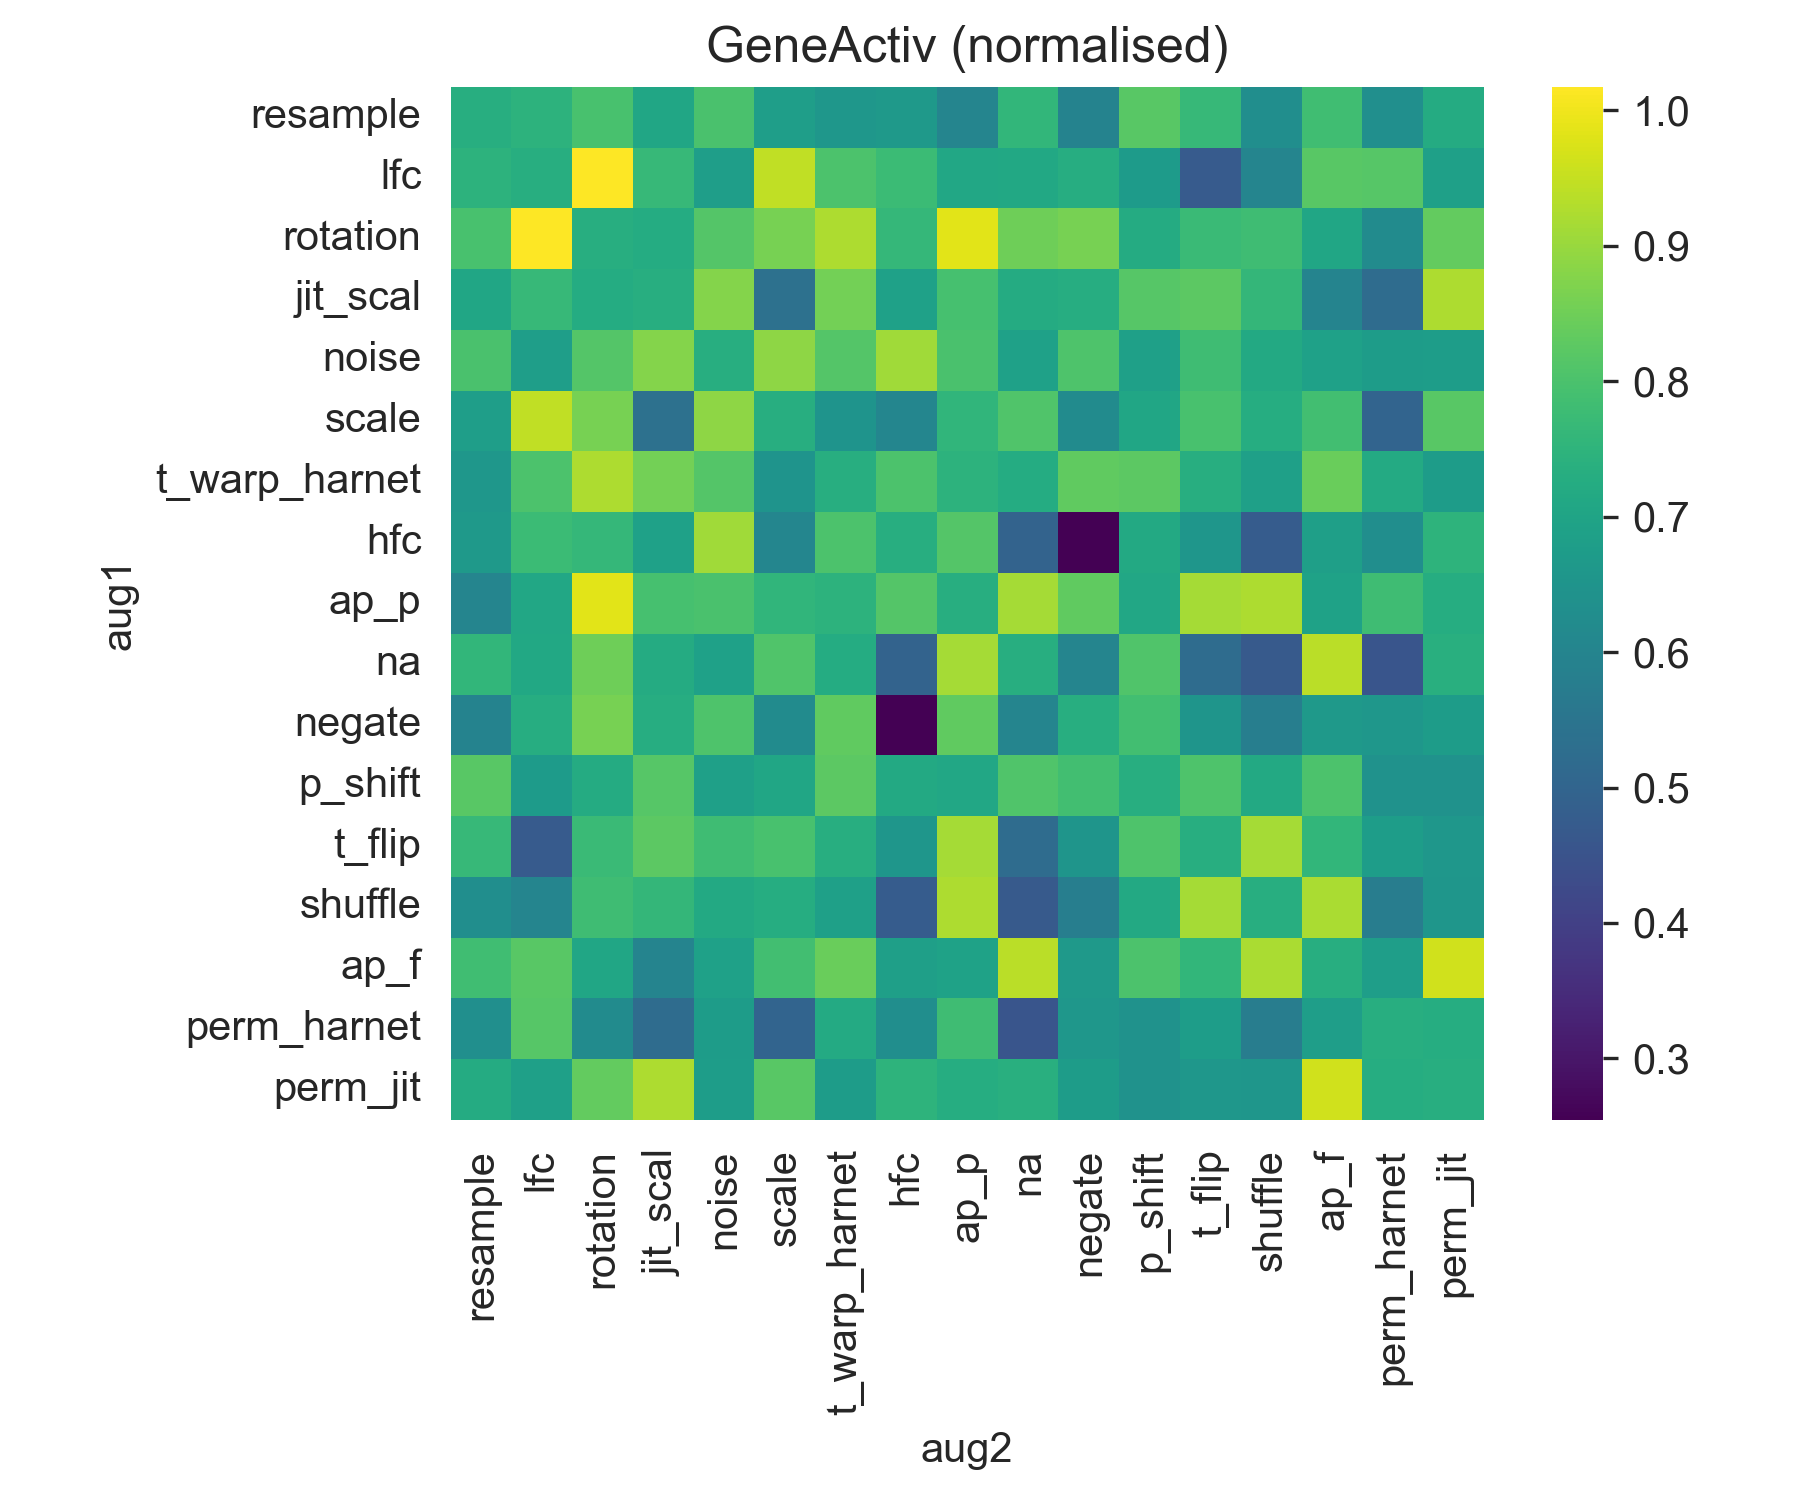
\includegraphics[width=\linewidth]{figures/geneactiv_normalised.png}  
  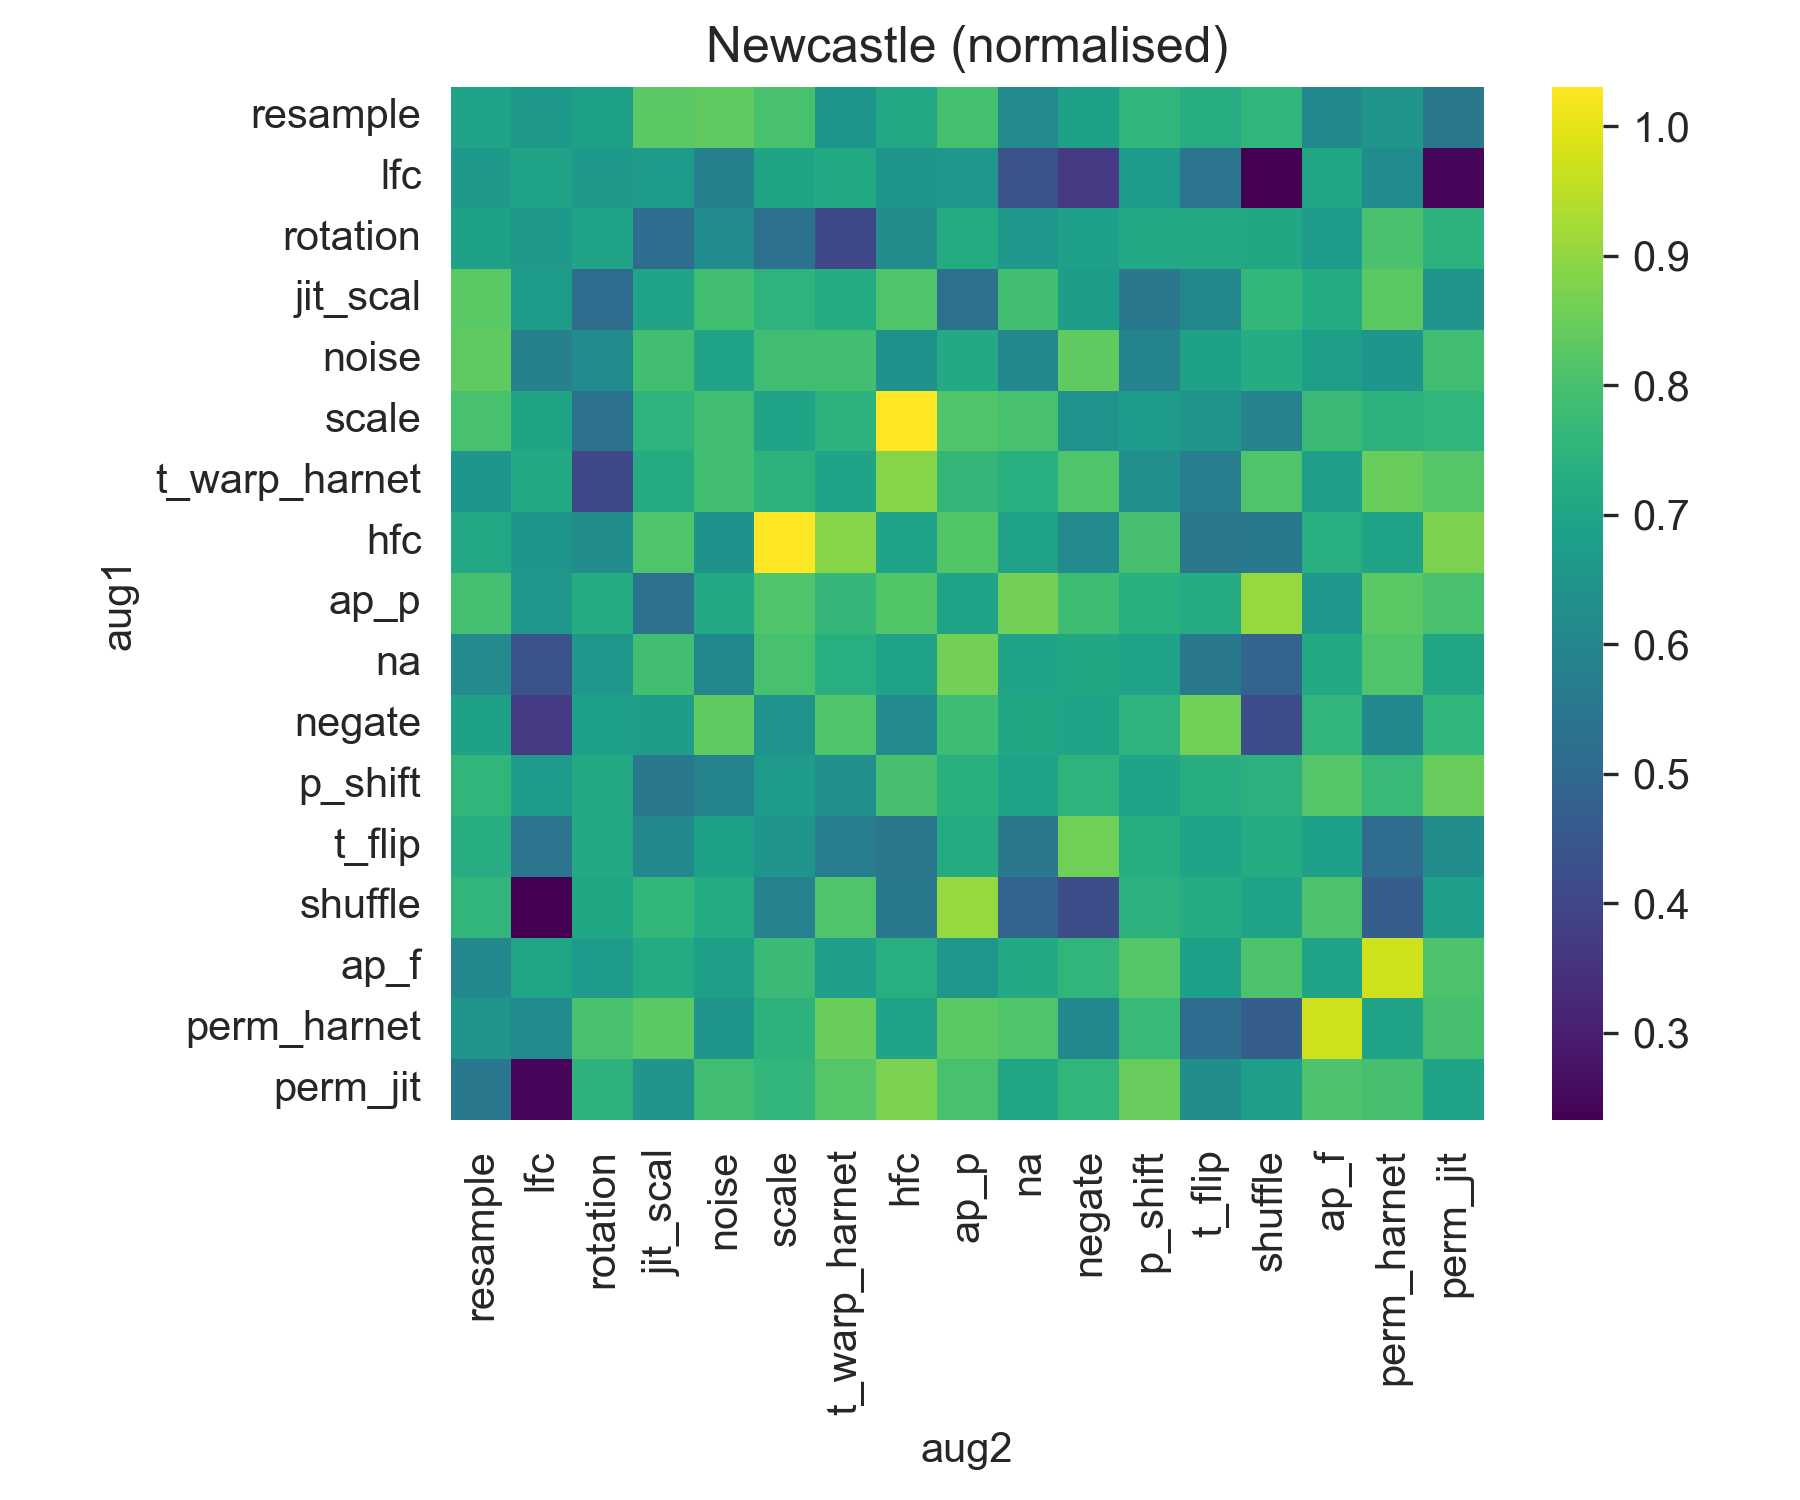
\includegraphics[width=\linewidth]{figures/newcastle_normalised.png}
  \caption{Caption text goes here.}
  \label{fig:example1}    
\end{figure}
\begin{table}[h]
\caption{Cross-validation Kappa Scores (Mean ± Std) per Dataset and Model}
\label{tab:kappa_scores}
\setlength{\tabcolsep}{1mm} % small padding
\begin{tabular}{|p{30mm}|p{17mm}|p{17mm}|p{17mm}|}
\hline
\textbf{Model} & 
\textbf{Applewatch} & 
\textbf{Geneactiv} & 
\textbf{Newcastle} \\
\hline
Harnet Capture24 & 
0.16 ± 0.07 & 
0.22 ± 0.04 & 
0.29 ± 0.08 \\
Harnet Capture24 \par (our method) & 
0.18 ± 0.08 & 
0.27 ± 0.05 & 
0.28 ± 0.08 \\
Harnet UKB & 
0.31 ± 0.09 & 
0.30 ± 0.04 & 
0.32 ± 0.09 \\
Our method & 
0.37 ± 0.08 & 
0.32 ± 0.06 & 
0.34 ± 0.08 \\
\hline
\multicolumn{4}{p{88mm}}{Values represent the mean and standard deviation of cross-validation Kappa scores across three datasets. All models were evaluated on the same folds for comparability.}
\end{tabular}
\end{table}


\section{Conclusion}
A conclusion section is not required. Although a conclusion may review the 
main points of the paper, do not replicate the abstract as the conclusion. A 
conclusion might elaborate on the importance of the work or suggest 
applications and extensions. 

\appendices

Appendixes, if needed, appear before the acknowledgment.

\section*{Acknowledgment}

The preferred spelling of the word ``acknowledgment'' in American English is 
without an ``e'' after the ``g.'' Use the singular heading even if you have 
many acknowledgments. Avoid expressions such as ``One of us (S.B.A.) would 
like to thank $\ldots$ .'' Instead, write ``F. A. Author thanks $\ldots$ .'' In most 
cases, sponsor and financial support acknowledgments are placed in the 
unnumbered footnote on the first page, not here.

\section*{References}
\bibliographystyle{IEEEtran} % or plain, unsrt, etc.
\bibliography{references}


\end{document}
